\subsection{Velocity map binning methods}
\label{sec:binning-methods}
The MaNGA DAP utilises various spaxel binning models to process the IFU fibre bundle data into the output maps. The available binning schemes used to produce gas and stellar velocity maps, together with a brief description of each are listed below.

\begin{itemize}
    \item SPX - single spaxel measurements i.e. no binning.
    \item VOR10 - Voronoi binning, an adaptive spatial binning method where low signal-to-noise (S/N) ratio spaxels are grouped to achieve an overall S/N of 10  \citep{2003MNRAS.342..345C, 2019arXiv190100856W}.
    \item HYB10 - Hybrid binning: Voronoi S/N 10 binning for stellar velocity maps, but unbinned for emission line properties which are used to generate gas velocity maps.
\end{itemize}  

In this study we have utilised MaNGA datacubes released in DR15 MPL-7 which have been processed in the DAP using the hybrid HYB10 binning model, i.e. using VOR10 binning for the stellar velocity maps. However, the MaNGA project team currently have an internal dataset available, MPL-8. Datacubes in MPL-8 include VOR10 and SPX binning schema. We were interested to make a comparison of the Radon trace profiles generated from the datacubes using the Voronoi and SPX binning schemas. A limited sample of MPL-8 cubes were made available for this comparison exercise. We selected 2 galaxies from our samples with stellar velocity maps having poor spatial definition, and another 2 with good resolution in order to compare the Radon transform profiles using the Voronoi binning and SPX (unbinned) methods. The selected datacubes were firstly, examples of good resolution/definition in stellar velocity maps:

\begin{itemize}
    \item 7977-12704
    \item 8322-1901
\end{itemize}

and secondly, examples of poor resolution/definition in stellar velocity maps, i.e. having a blotchy appearance, due to spatial binning of low S/N spaxels, or with masked spaxels:

\begin{itemize}
    \item 9088-12703
    \item 8993-6104
\end{itemize}

The stellar velocity maps together with their Radon transform and trace profiles for these well defined example 7977-12704 are shown in Figure \ref{fig:binning-comparison}. The differences being the binning models of the input stellar velocity maps: Voronoi binning in the left-hand panel and SPX binning on the right. A comparison shows that there is little difference in the Radon transform and Radon profile plots. It is also apparent that the Radon transform algorithm for the SPX velocity maps yields a greater number of valid data points in the trace plot. We conclude that both VOR10 and SPX binned maps would lead to the same Type classification in these cases. This conclusion was also obtained for other galaxy showing good resolution in the stellar velocity map,  8322-1901 (figure not included). 

However, the same conclusion does not apply for the low resolution stellar velocity map examples, 8993-6104 shown in Figure \ref{fig:binning-comparison2} and 9088-12703 (figure not included). In these cases, at first sight, there are marked differences in the extent of spatial coverage and shapes of the velocity field PA, the Radon transform minimum and the Radon profile. In particular the control galaxy 8993-6104 displays a clearly asymmetric Radon profile with VOR10 binning, but could possibly be interpreted as an outer bend in the Radon profile trace of the SPX map. However, on closer inspection, looking at the  range the trace plots, the same bend feature at Radon transform coordinates [$\rho$, $\theta$]=[-6,+2],[20, 50] is apparent in both binning model plots. The asymmetric feature at $\rho$ \textgreater\ +2 apparent in the left Voronoi binned trace is not evident in the SPX output shown in the right-hand panel. Although these differences can be expected due to the exclusion of low S/N low spaxels in the SPX maps, crucially this can easily lead to a different visual classification result between the transforms of Voronoi binned and SPX velocity field maps. 
\begin{figure*}
    \centering
    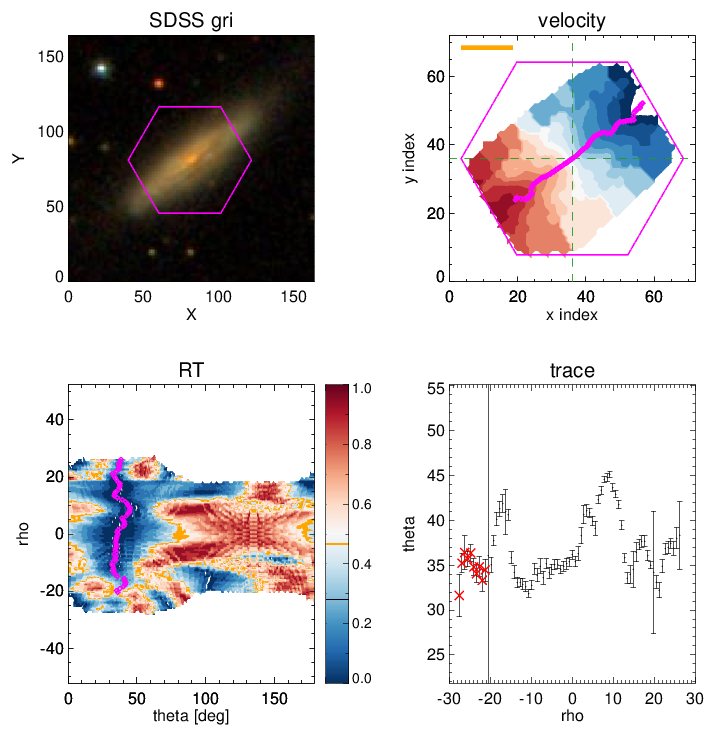
\includegraphics[width=\columnwidth]{images/RadonPlots/RT-SNIPS-NEW/7977-12704-VOR10-MILESHC-MILESHC-1-SNIP.png}
    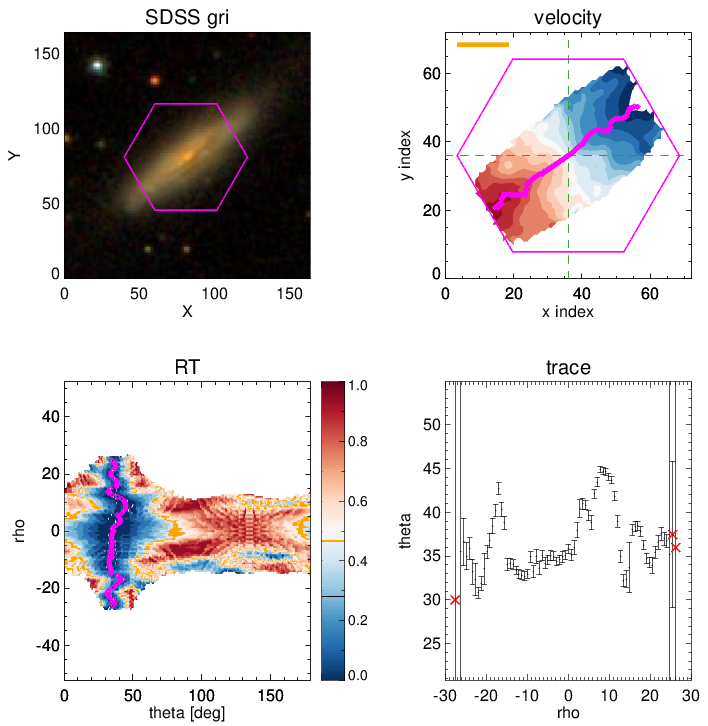
\includegraphics[width=\columnwidth]{images/RadonPlots/RT-SNIPS-NEW/7977-12704-SPX-MILESHC-MILESHC-1-SNIP.png}
    \caption[Comparison of velocity map binning schemes for a high resolution map]{Comparison of stellar velocity map binning methods using the Radon transform output graphic for the galaxy 7977-12704. The velocity map has good resolution using both schemes. In the left panel the transform RT and profile trace plots are generated from the stellar velocity map with Voronoi binning. The plots in the right panel were produced from the stellar velocity map using single spaxel SPX resolution. The layout of the 4 subplots in each panel is as described in Figure \ref{fig:8442-3704-complete}.}
    \label{fig:binning-comparison}
\end{figure*}

\begin{figure*}
    \centering
    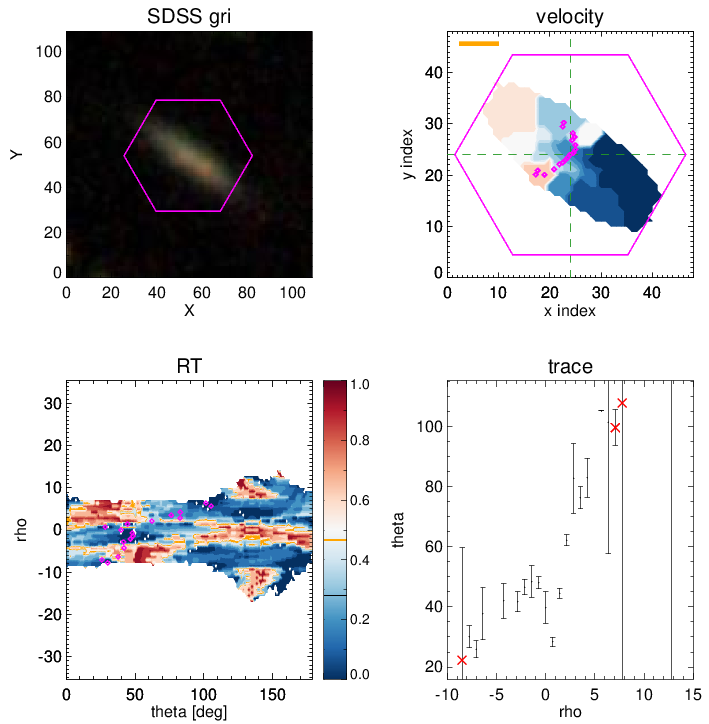
\includegraphics[width=\columnwidth]{images/RadonPlots/RT-SNIPS-NEW/8993-6104-VOR10-MILESHC-MILESHC-1-SNIP.png}
    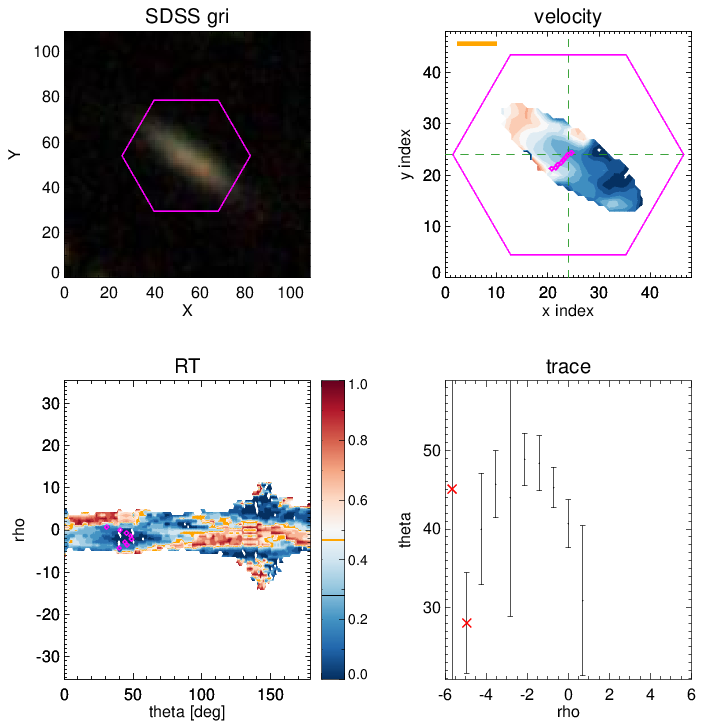
\includegraphics[width=\columnwidth]{images/RadonPlots/RT-SNIPS-NEW/8993-6104-SPX-MILESHC-MILESHC-1-SNIP.png}
    \caption[Comparison of velocity map binning schemes for a low resolution map]{Comparison of velocity map binning schemes for a low resolution map. Radon transform output graphic for the galaxy 8993-6104 with a low resolution stellar velocity map. In the left panel the transform RT and profile trace plots are generated from the stellar velocity map with Voronoi binning. The plots in the right panel were produced from the stellar velocity map using single spaxel SPX binning. The layout of the 4 subplots in each panel is as described in Figure \ref{fig:8442-3704-complete}.}
    \label{fig:binning-comparison2}
\end{figure*}


